\section{Pumped cavity}
The derivation for the Hamiltonians for the following sections is taken from \cite{donner}.

\subsection{Longitudinal Pump}
In the simulation we set the external Potential to 0. We set $U_0 \coloneqq g_0^2/\Delta a$. Since we are working with a red-detuned laser, $\Delta a$ and $\Delta c$ are smaller 0. The Hamiltonian is:

\begin{align}
H_\text{long} = \frac{p^2}{2m} + V_\text{ext}(x) - \hbar \Delta_c a^\dagger a + \hbar \eta (a + a^\dagger) + \hbar U_0 \cos(kx)^2 a^\dagger a.
\end{align}We want to make sure all quantities are expressed with the recoil energy $E_r = \hbar \omega_r$, where $\omega_r = \hbar k^2 / 2m$ is the recoil frequency. Therefore we factor our $E_r$ to see what we have to type into the program:

\begin{align}
\begin{split}
H_\text{long} = \hbar \omega_r \biggl( \frac{1}{\hbar^2 k^2} p^2 + \frac{1}{\hbar \omega_r} V_\text{ext}(x) - \frac{1}{\omega_r} \Delta_c a^\dagger a + \frac{1}{\omega_r} \eta (a + a^\dagger) + \\
 + \frac{1}{\hbar \omega_r} U_0 \cos(kx)^2 a^\dagger a \biggr).
\end{split}
\end{align}In the simulation program, we will thus set $\hbar = 1$ and divide each quantity by the preceding factors.

\subsection{Transversal pump}
Again, in the simulation we set the external potential to 0. Here we only consider one dimension, so we set $z=0$.

\begin{align}
\begin{split}
H_\text{transv} = \frac{p^2}{2m} + V_\text{ext}(x) - \hbar \Delta_c a^\dagger a - \hbar \eta \cos(kx) \cos(kz) (a + a^\dagger) + \\
 + \hbar U_0 \cos(kz)^2 + \hbar U_0 \cos(kz)^2 a^\dagger a.
\end{split}
\end{align}As previously mentioned, keeping the right dimensionality in the simulation is very important.

\section{Results}
The longitudinal spatial wave function densities are depicted in Figure~\ref{long_eta} for different values of $\eta$.

\begin{figure}[htp]
\centering
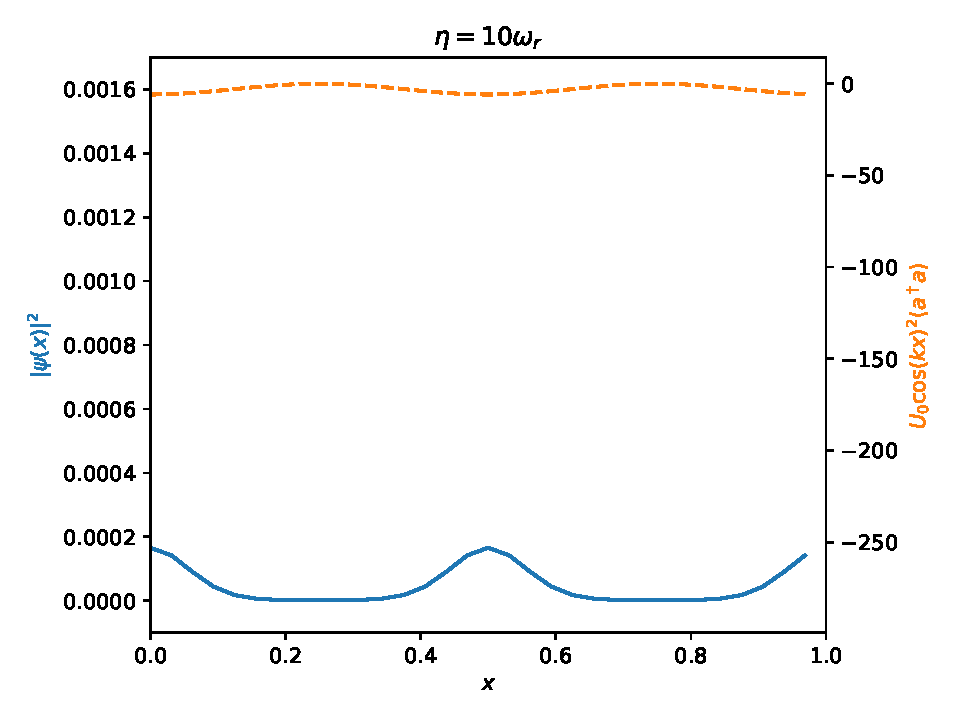
\includegraphics[width=.3\textwidth]{long_eta_10.pdf}\hfill
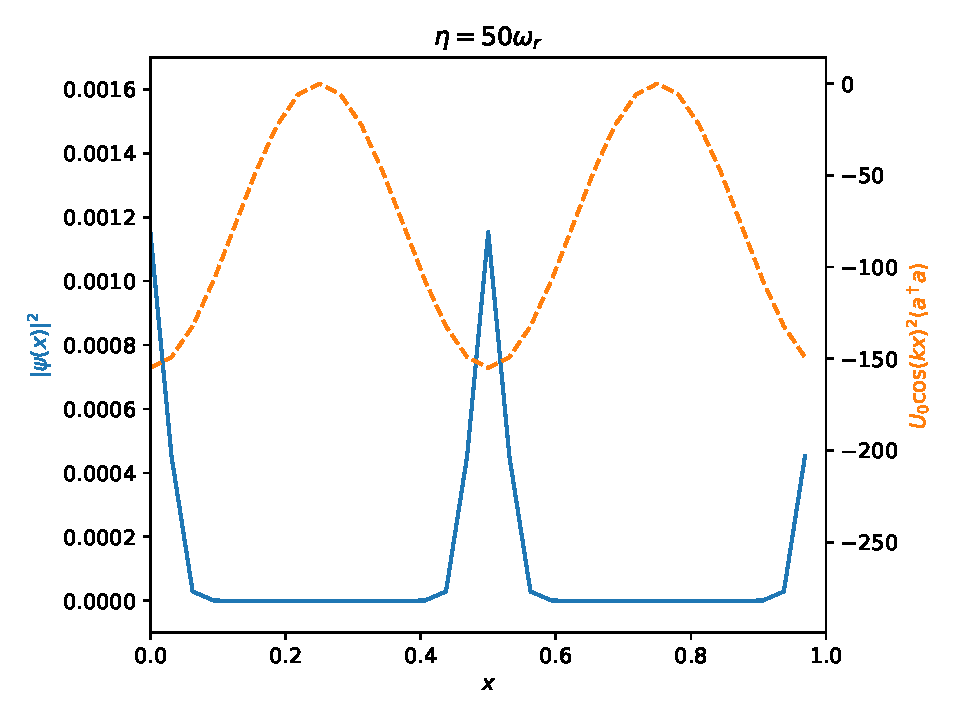
\includegraphics[width=.3\textwidth]{long_eta_50.pdf}\hfill
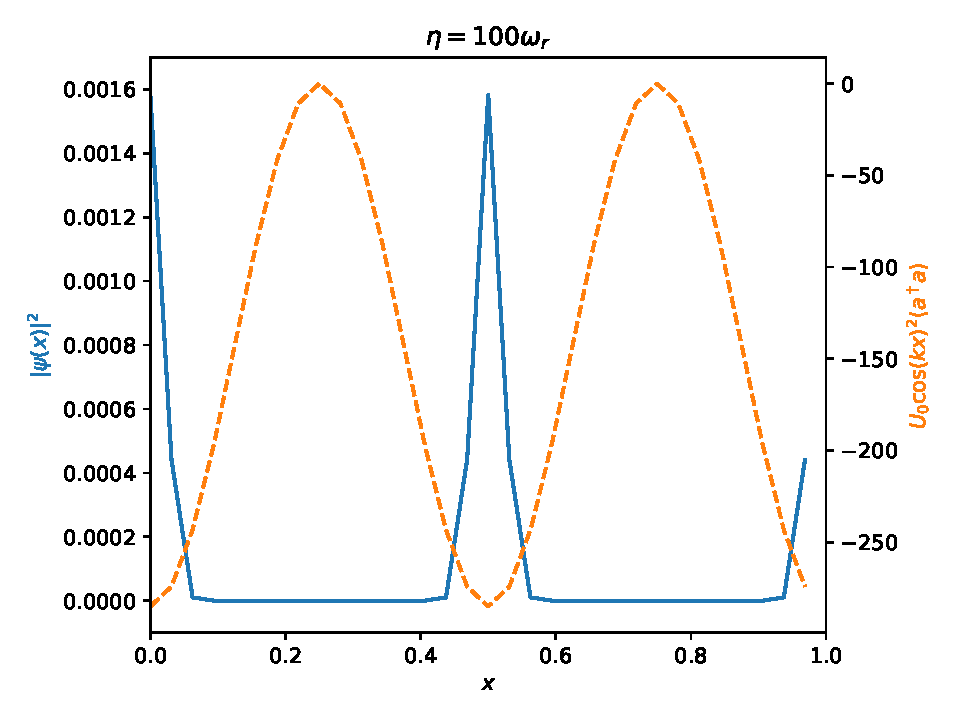
\includegraphics[width=.3\textwidth]{long_eta_100.pdf}
\caption{Longitudinal wave function densities for $\eta = 10 \omega_r$, $\eta = 50 \omega_r$ and $\eta = 100 \omega_r$.}
\label{long_eta}
\end{figure}
\FloatBarrier

\noindent Figures \ref{long_pmp_bunch} and \ref{trans_pmp_bunch} depict the bunching parameter $\langle \cos(kx)^2 \rangle$ each. We did not obtain any meaningful results with the order parameter $\langle \cos(kx) \rangle$.

\begin{figure}[ht]
  \centering
  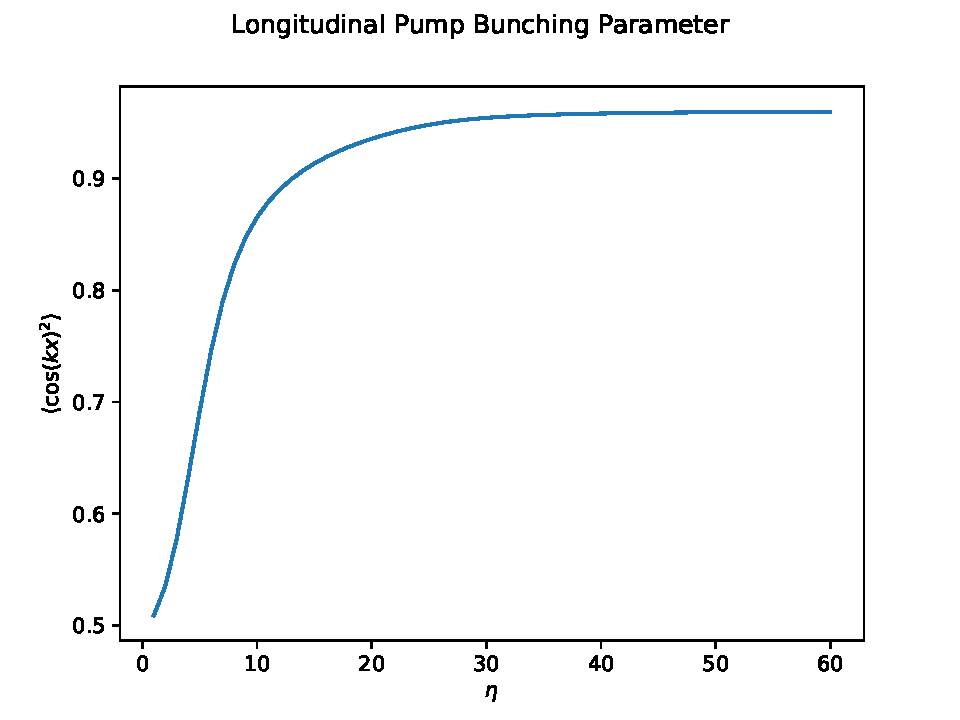
\includegraphics[width=.7\linewidth]{long_pmp_bunch.pdf}
  \caption{Bunching parameter for longitudinal pump with $\Delta_c = -10 \omega_r$ and $U_0 = -1 \omega_r$.}
  \label{long_pmp_bunch}
\end{figure}
\FloatBarrier

\begin{figure}[ht]
  \centering
  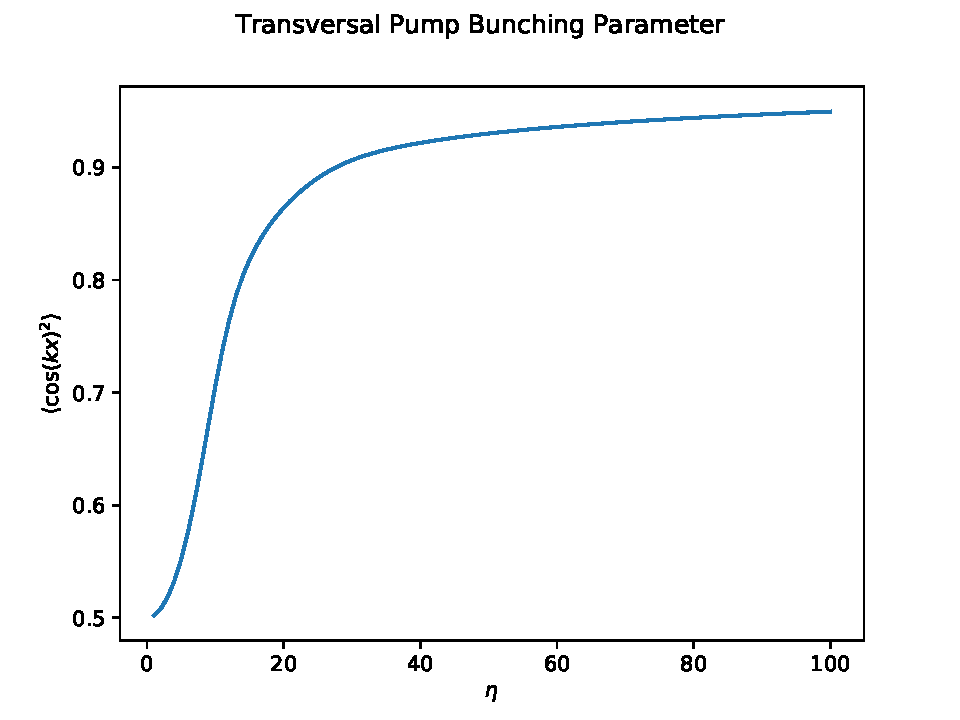
\includegraphics[width=.7\linewidth]{trans_pmp_bunch.pdf}
  \caption{Bunching parameter for transversal pump with $\Delta_c = -10 \omega_r$ and $U_0 = -1 \omega_r$.}
  \label{trans_pmp_bunch}
\end{figure}
\FloatBarrier

\noindent To obtain the order parameter as a function of $\eta$ for transversal pump, we used the mean-field approximation, as depicted in \cite{cold_atoms}. For now, a simple Euler algorithm will do. The results can be seen in Figure~\ref{trans_pmp_order}. Strangely, there is no threshold at which order sets in, but rather a gradual shift. We also tried to tweak the parameters similar to \cite{Nagy2008}, which unfortunately made the wave function all but disappear.

\begin{figure}[ht]
  \centering
  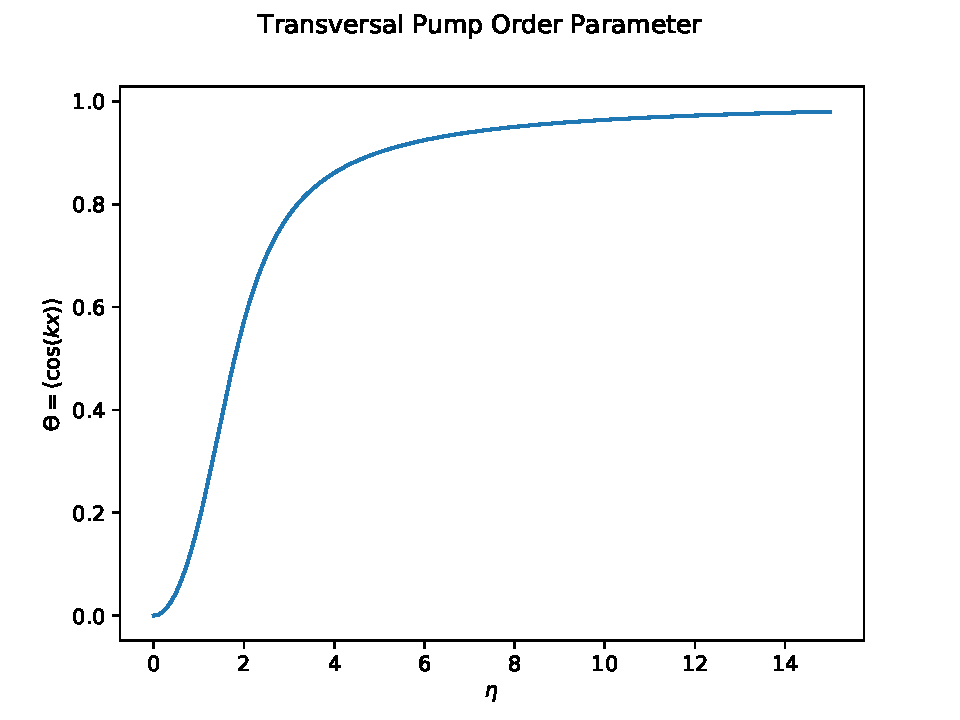
\includegraphics[width=.7\linewidth]{trans_pmp_order.pdf}
  \caption{Order parameter for transversal pump with $\Delta_c = -1 \omega_r$, $U_0 = -1 \omega_r$ and $\kappa = \omega_r$.}
  \label{trans_pmp_order}
\end{figure}
\FloatBarrier